%
%  MAIN driver/organizer for slide presentation
%

\documentclass[aspectratio=169]{beamer}

%%
\makeatletter
\defbeameroption{show only notes}[]% 
{
\beamer@notestrue
\beamer@notesnormalsfalse
}
\makeatother

\setbeameroption{hide notes}

%%  ... include packages

% !TEX root = ../digraph-main.tex
% packages.tex

\usetheme{Madrid}
\usepackage{appendixnumberbeamer}
\usefonttheme[onlymath]{serif}

% \usepackage{pgfplots}
%\usepackage{chronosys}

% fix booktabs compatibility issue
%\usepackage{etex}
%\usepackage{animate}

% math
%\usepackage{sansmathaccent}
\usepackage{amsmath}
\usepackage{amssymb}
\usepackage{amsthm}                 % Theorems/definitions
%\usepackage{mathrsfs}
\usepackage{array}
\usepackage{mathtools}

% SI units
\usepackage[detect-all]{siunitx}

% graphics
\usepackage[compatibility=false,justification=raggedright,
            font=scriptsize,labelformat=empty,skip=0pt,
            singlelinecheck=true]{caption}
\usepackage[labelformat=empty,justification=raggedright]{subcaption}
% \usepackage{graphicx}

\usepackage{xparse,fp}
%\usepackage{datenumber,xparse,fp}
\usepackage{pgf}
\usepackage{tikz}
\usetikzlibrary{arrows.meta}
\usetikzlibrary{decorations.text}
\usetikzlibrary{automata, positioning}
\usetikzlibrary{backgrounds}
\usetikzlibrary{tikzmark}
\usetikzlibrary{calc}
\usepackage{adjustbox}

% tables
\usepackage{multirow}
\usepackage{booktabs}
%\usepackage{colortbl}
%\usepackage{diagbox}
%\usepackage{arydshln} % dash line in tables
%\usepackage{makecell}
\usepackage{scalerel}

% clever references
\usepackage{cleveref}

% fonts
%% \usepackage{sfmath}
\usepackage{textcomp}
%\usepackage[resetfonts]{cmap}
\usepackage[utf8]{inputenc}
% \usepackage{natbib}

\usepackage[hyperref=true,
            url=false,
            isbn=false,
            backref=false,
            doi=false,
            style=authoryear,
            firstinits=true,
            citereset=section,
            maxcitenames=1,
            maxbibnames=100,
            backend=bibtex, % while checking on one of my (newest) systems, this option was needed to generate bibliography
            block=none]{biblatex}

\usepackage[T1]{fontenc}
\usepackage{amsmath}

%\usepackage{fancybox} 
%\usepackage{framed,color}

% algorithm listing
\usepackage[noend]{algorithm2e}

% lists
% \usepackage{paralist}
\usepackage{enumerate}


%\usepackage[export]{adjustbox}


% fix cref
\crefname{proposition}{Proposition}{Propositions}
\Crefname{proposition}{Proposition}{Propositions}

\usepackage{bm}


% !TEX root = ../digraph-main.tex
% customization.tex


\definecolor{applegreen}{rgb}{0.55, 0.71, 0.0}
\definecolor{dukeblue}{RGB}{0, 83, 155}
\definecolor{navyblue}{RGB}{1, 33, 105}

\setbeamercolor{frametitle}{bg=navyblue, fg=white}
% \setbeamertemplate{section in toc}[sections numbered]
% \setbeamertemplate{subsection in toc}[subsections numbered]
% \useoutertheme[subsection=false]{miniframes}
% \setbeamercolor{section in head/foot}{fg=white, bg=dukeblue}
% \setbeamerfont{section in head/foot}{series=\bfseries}

% \makeatletter
% \setbeamertemplate{frametitle}{%
%   \nointerlineskip%
%   \begin{beamercolorbox}[%
%       wd=\paperwidth,%
%       sep=0pt,%
%       leftskip=\metropolis@frametitle@padding,%
%       rightskip=\metropolis@frametitle@padding,%
%       ht=2.25ex,%%%%%% NEW !!!!!!!!!!!!!!!!!!!!!!!!!!!!!!!!!!!!!!!!
%       dp=1.1ex, %%%%%% NEW !!!!!!!!!!!!!!!!!!!!!!!!!!!!!!!!!!!!!!!!
%     ]{frametitle}%
%   \metropolis@frametitlestrut@start%
%   \insertframetitle%
%   \nolinebreak%
%   \metropolis@frametitlestrut@end%
%   \end{beamercolorbox}%
% }
% \makeatother

% get rid of navigation symbols
\setbeamertemplate{navigation symbols}{}

% remove shadow from title block
\setbeamertemplate{title page}[default][colsep=-4bp,rounded=true]

% use square-type bullets
\setbeamertemplate{itemize item}[circle]
\setbeamertemplate{itemize subitem}{--}
\setbeamertemplate{enumerate item}[circle]

% use circles for ToC items and correct the weird size issue with "Madrid" theme
\setbeamertemplate{sections/subsections in toc}[circle]
\setbeamerfont{section number projected}{size=\normalsize}

% figure captions: no "figure" prefix, small text, small figure-caption space
\captionsetup[figure]{labelformat=empty}
\captionsetup[table]{labelformat=empty}
\captionsetup[figure]{font=tiny,labelfont=tiny}
\captionsetup[subfigure]{font=tiny,labelfont=tiny}

% command for fixing inline TikZ nodes' vertical alignment
\newcommand{\tikzbasefix}{-\the\dimexpr\fontdimen22\textfont2\relax}

% define coloured clickable links
\hypersetup{%
  pdffitwindow=false,%
  pdfstartview={FitH},%
  % colorlinks,%
  pdfauthor={},%
  pdftitle={},%
  pagebackref=true,%
  citecolor=PaleGreen4,%
  filecolor=DarkOrchid4,%
  % linkcolor=OrangeRed4,%
  urlcolor=RoyalBlue4%
}

% define the includegraphics search path
\graphicspath{%
  {./figures/}%
}

% short-hand command for hyperlinked e-mails
\newcommand{\email}[1]{\href{mailto:#1}{\texttt{#1}}}

% customize TikZ matrix column separator character (to avoid Beamer
% conflict)
\tikzset{ampersand replacement=\&}

% redefine \boxed command to allow setting the border color
\newcommand{\highlight}[1]{\fcolorbox{complclr1}{white}{$\displaystyle #1$}}

% remove extra spacing around \left and \right delimiters
\let\leftorig\left
\let\rightorig\right
\renewcommand{\left}{\mathopen{}\mathclose\bgroup\leftorig}
\renewcommand{\right}{\aftergroup\egroup\rightorig}

% increase vertical spacing between table rows
\renewcommand{\arraystretch}{1.2}

% modified bullet-point for highlighting
\newcommand{\bulletemph}{$\large\boldsymbol{\star}$}

% superscript comma for footnote references
\newcommand{\footcomma}{\textsuperscript{,}}

% command to output names under images
\newcommand{\imentry}[3][1.25cm]{%
  \vbox{\halign{\hfil##\hfil\cr%
      \includegraphics[height=#1]{#2}\cr#3\cr}}}

% pictures goes with authors
\newcommand{\theauthor}[2]{\vbox{\halign{\hfil##\hfil\cr
  \includegraphics[width=0.125\textwidth]{#1}\cr#2\cr}}}

\newcommand{\theauthornopic}[1]{\vbox{\halign{\hfil##\hfil\cr
  \cr#1\cr}}}

\DeclareCaptionFont{tiny}{\tiny}

\newcommand{\backupbegin}{
   \newcounter{finalframe}
   \setcounter{finalframe}{\value{framenumber}}
}
\newcommand{\backupend}{
   \setcounter{framenumber}{\value{finalframe}}
}

\setbeamerfont{footnote}{size=\tiny}

% timeline option
\newlength\yearposx

% fix bug in beamer
% [https://tex.stackexchange.com/a/426090]
\makeatletter
\let\@@magyar@captionfix\relax
\makeatother

% alternative footnote by Tiancheng Liu
\newcommand\alternativefootnote[1]{%
 \tikz[remember picture,overlay]
 \draw (current page.south west) +(1in + \oddsidemargin,1em)
 node[anchor=south west,inner sep=0pt]{\parbox{\textwidth}{%
     \rlap{\rule{10em}{0.4pt}}\raggedright\tiny#1}};}


\def\signed #1{{\leavevmode\unskip\nobreak\hfil\penalty50\hskip1em
    \hbox{}\nobreak\hfill #1%
    \parfillskip=0pt \finalhyphendemerits=0 \endgraf}}

\newsavebox\mybox
\newenvironment{aquote}[1]
{\savebox\mybox{#1}\begin{quote}\hspace*{-.7ex}}
  {\unskip\vspace*{1mm}\signed{\usebox\mybox}\end{quote}}


% define new table columns for fixed-width center columns
% 
% [https://tex.stackexchange.com/a/12712]
\newcolumntype{C}[1]{>{\centering\let\newline\\\arraybackslash\hspace{0pt}}m{#1}}

% change how sections and subsection are highlight in TOC
\setbeamertemplate{section in toc}{
  \textbf{\inserttocsectionnumber.~\inserttocsection}}
\setbeamertemplate{section in toc shaded}{
  \inserttocsectionnumber.~\inserttocsection}

\setbeamertemplate{subsection in toc}{
  \hspace{1.2em}{\rule[0.3ex]{3pt}{3pt}}~\textbf{\inserttocsubsection}\par}
\setbeamertemplate{subsection in toc shaded}{
  \hspace{1.2em}{\rule[0.3ex]{3pt}{3pt}}~\inserttocsubsection\par}

% clever ref
\crefname{equation}{}{}
\Crefname{equation}{}{}

% extra rule for adding image with raggedright centered caption
\newcommand{\lcaption}[2]{ %
  % 
  \captionsetup{justification=raggedright}
  % 
  \begin{minipage}{#1}
    \caption{ %
      #2
    }
  \end{minipage}
}

\DeclareSIUnit{\nothing}{\relax}

\newcommand*{\textcal}[1]{%
  % family qzc: Font TeX Gyre Chorus (package tgchorus)
  % family pzc: Font Zapf Chancery (package chancery)
  \textbf{\textit{\fontfamily{qzc}\selectfont#1}}% 
}

\DeclareMathAlphabet{\zcal}{\encodingdefault}{sqzc}{m}{it}


\addtobeamertemplate{frametitle}{}{\vspace*{-0.5em}}


\newcommand{\gls}{G$\ell$S}

\newcommand{\conf}{\Omega}

\newcommand{\ha}{h_{\rm a}}
\newcommand{\hr}{h_{\rm r}}
\newcommand{\dm}{{{\em d.m.}}}

\newcommand{\bluered}{br}

\setbeamercolor{block body}{bg=dukeblue!30}
\setbeamercolor{block title}{bg=dukeblue,fg=black!2}


% theorem and collorary
\setbeamertemplate{theorems}[numbered] 

\makeatletter
\g@addto@macro\normalsize{%
    \setlength\abovedisplayskip{2pt}
}
\g@addto@macro\normalsize{%
    \setlength\belowdisplayskip{2pt}
}

\newcommand{\smsp}{\mspace{2mu}}  % slightly smaller space than \,
\DeclareMathOperator*{\argmax}{arg \smsp max}
\DeclareMathOperator*{\argmin}{arg \smsp min}

\newtheorem{proposition}{Proposition}


\def\arrowtext#1#2{\hbox to#1{\arrowtextA\ #2 \arrowtextA\kern2pt\llap{$\succ$}}}
\def\arrowtextA{\leaders\vrule height2.7pt depth-2.3pt\hfil}

\newcommand{\tikzvrule}[1]{
  \draw   ([yshift=-0.8cm,xshift=#1]current page.north west)
       -- ([xshift=#1]current page.south west)
}

\newcommand{\tikzvsubrule}[3]{
  \draw   ([yshift=-0.8cm+#2,xshift=#1]current page.north west)
       -- ([yshift=-0.8cm+#3,xshift=#1]current page.north west)
}

\newcommand{\tikzhrule}[1]{
  \draw   ([yshift=-0.8cm+#1]current page.north west)
       -- ([yshift=-0.8cm+#1]current page.north east)
}

\newcommand{\tikzhsubrule}[3]{
  \draw   ([yshift=-0.8cm+#1,xshift=#2]current page.north west)
       -- ([yshift=-0.8cm+#1,xshift=#3]current page.north east)
}


% footnote size & enable footnotes
% \renewcommand{\footnotesize}{\fontsize{5pt}{8pt}\selectfont}
% \let\oldfootnote\footnote
% \renewcommand\footnote[1][]{\oldfootnote[frame,#1]}

\renewcommand*{\bibfont}{\tiny}

% \AtEveryCitekey{
% %   \clearfield{location}
%   \clearfield{title}
%   \clearfield{number}
%   \clearfield{volume}
% %   \clearfield{publisher}
% }

\renewbibmacro*{cite}{%
  \iffieldundef{shorthand}
    {\ifthenelse{\ifnameundef{labelname}\OR\iffieldundef{labelyear}}
       {\usebibmacro{cite:label}%
        \setunit{\printdelim{nonameyeardelim}}}
       {\printnames{labelname}%
        \setunit{\printdelim{nameyeardelim}}}%
     \usebibmacro{cite:labeldate+extradate}%
     \setunit{\addcomma\space}%
     \usebibmacro{journal}}
   {\usebibmacro{cite:shorthand}}}

\setbeamertemplate{bibliography item}{}

%\makeatletter
%\newcommand{\xleftrightarrow}[2][]{\ext@arrow 3359\leftrightarrowfill@{#1}{#2}}
%\makeatother


% !TEX root = ../digraph-main.tex
% graphics.tex


% ---------- colors ---------- %

% color palette
\definecolor{baseclr}{HTML}{27408B}
\definecolor{myclr}{HTML}{000000}
\definecolor{complclr}{HTML}{CE9927}

% 2 complementary color sets
\definecolor{myblue}{HTML}{27408B}
\definecolor{myorange}{HTML}{CE9927}
\definecolor{myred}{HTML}{A92066}
\definecolor{mygreen}{HTML}{86BF24}

% alternative green-red combination
\definecolor{otherred}{HTML}{AA3939}
\definecolor{othergreen}{HTML}{2E882E}

% beamer colors
\setbeamercolor{normal text}{fg=baseclr}
\setbeamercolor{section in toc}{fg=baseclr}
\setbeamercolor{subsection in toc}{fg=baseclr}

% shade colors & listings

\definecolor{lightgray}{gray}{0.95} 
\definecolor{shadecolor}{rgb}{0.95,0.95,0.85}    % weights by xiaobai 

\sloppy



% !TEX root = ../digraph-main.tex
% extras.tex


\usetheme{Madrid}
\setbeamertemplate{caption}[numbered]
\setbeamertemplate{caption label separator}{: }
\setbeamercolor{caption name}{fg=normal text.fg}
\usepackage{lmodern}
\usepackage{amssymb,amsmath}
\usepackage{ifxetex,ifluatex}
\usepackage{fixltx2e} % provides \textsubscript
\ifnum 0\ifxetex 1\fi\ifluatex 1\fi=0 % if pdftex
  \usepackage[T1]{fontenc}
  \usepackage[utf8]{inputenc}
\else % if luatex or xelatex
  \ifxetex
    \usepackage{mathspec}
  \else
    \usepackage{fontspec}
  \fi
  \defaultfontfeatures{Mapping=tex-text,Scale=MatchLowercase}
  \newcommand{\euro}{€}
\fi
% use upquote if available, for straight quotes in verbatim environments
\IfFileExists{upquote.sty}{\usepackage{upquote}}{}
% use microtype if available
\IfFileExists{microtype.sty}{%
\usepackage{microtype}
\UseMicrotypeSet[protrusion]{basicmath} % disable protrusion for tt fonts
}{}
\usepackage{listings}
\usepackage{graphicx,grffile}
\makeatletter
\def\maxwidth{\ifdim\Gin@nat@width>\linewidth\linewidth\else\Gin@nat@width\fi}
\def\maxheight{\ifdim\Gin@nat@height>\textheight0.8\textheight\else\Gin@nat@height\fi}
\makeatother
% Scale images if necessary, so that they will not overflow the page
% margins by default, and it is still possible to overwrite the defaults
% using explicit options in \includegraphics[width, height, ...]{}
\setkeys{Gin}{width=\maxwidth,height=\maxheight,keepaspectratio}

% Comment these out if you don't want a slide with just the
% part/section/subsection/subsubsection title:
% \AtBeginPart{
%   \let\insertpartnumber\relax
%   \let\partname\relax
%   \frame{\partpage}
% }
%\AtBeginSection{
%  \let\insertsectionnumber\relax
%  \let\sectionname\relax
%  \frame{\sectionpage}
%}
%\AtBeginSubsection{
%  \let\insertsubsectionnumber\relax
%  \let\subsectionname\relax
%  \frame{\subsectionpage}
%}

% show plan before each section
% \AtBeginSection[]
% {
%   \begin{frame}[noframenumbering,plain]
%     % \frametitle{Outline}
%     \tableofcontents[currentsection,
%         currentsubsection,
%         subsectionstyle=show/show/hide]
%   \end{frame}
% }

\setlength{\emergencystretch}{3em}  % prevent overfull lines
\providecommand{\tightlist}{%
  \setlength{\itemsep}{0pt}\setlength{\parskip}{0pt}}
\setcounter{secnumdepth}{0}

%% ============ set up the title slide and footer information

% title.tex


\title%
[Short title (footer)]%                                %%  short version for footer
{Long title (frontmatter, title slide)}%             %%  long version

% \subtitle                                                                      %% used for location and time of presentation
% {\vspace*{0.5em}\footnotesize
%     \\
%   Oct.   2021
% }

% -------------------- AUTHOR LIST ( & short info in FOOTER )

\author%
[Dimitris Floros]%                                    %% including photos and short info for FOOTER
{%
  % \theauthornopic{Dimitris Floros\footnotemark[1]}  %% without picture
  \theauthor{authors/XS}{Xiaobai Sun\footnotemark[1]}
  \theauthor{authors/NP}{Nikos Pitsianis}
  \theauthor{authors/DF}{Dimitris Floros\footnotemark[1]}
  \theauthor{authors/TL}{Tiancheng Liu}
}

\institute%
[Duke]% % short for FOOTER info
{%
  \inst{1}
  Duke University, NC, USA%, 
}

\date%
[\today]%
{\today}


% ========== bibliography
\bibliography{ref.bib}

\begin{document}


\frame{\titlepage}                     % the very first slide frame 

\begin{frame}[noframenumbering,plain]
  \frametitle{Outline}
  \tableofcontents
\end{frame}

%%  ---------- Outline 
% \part{Part I}

\section{First section (use sections for outline)}

% simple.tex
%
% Drafted by Dimitris on August 21, 2022
%

\begin{frame}
  \frametitle{Citing articles}

  A demo cite


  \alternativefootnote{
    \cite{barabasi1999}; \cite{barabasi1999}
  }

\end{frame}

%%% Local Variables:
%%% mode: latex
%%% TeX-master: "../topic-slide-main"
%%% End:


%% ----------- Problem description 

% % problem-description.tex
% Drafted by Juntang on September 10, 2024
%

\begin{frame}{Problem description}
    \begin{columns}
        % Left column
        \begin{column}{0.38\textwidth}
            \begin{figure}
            \centering
            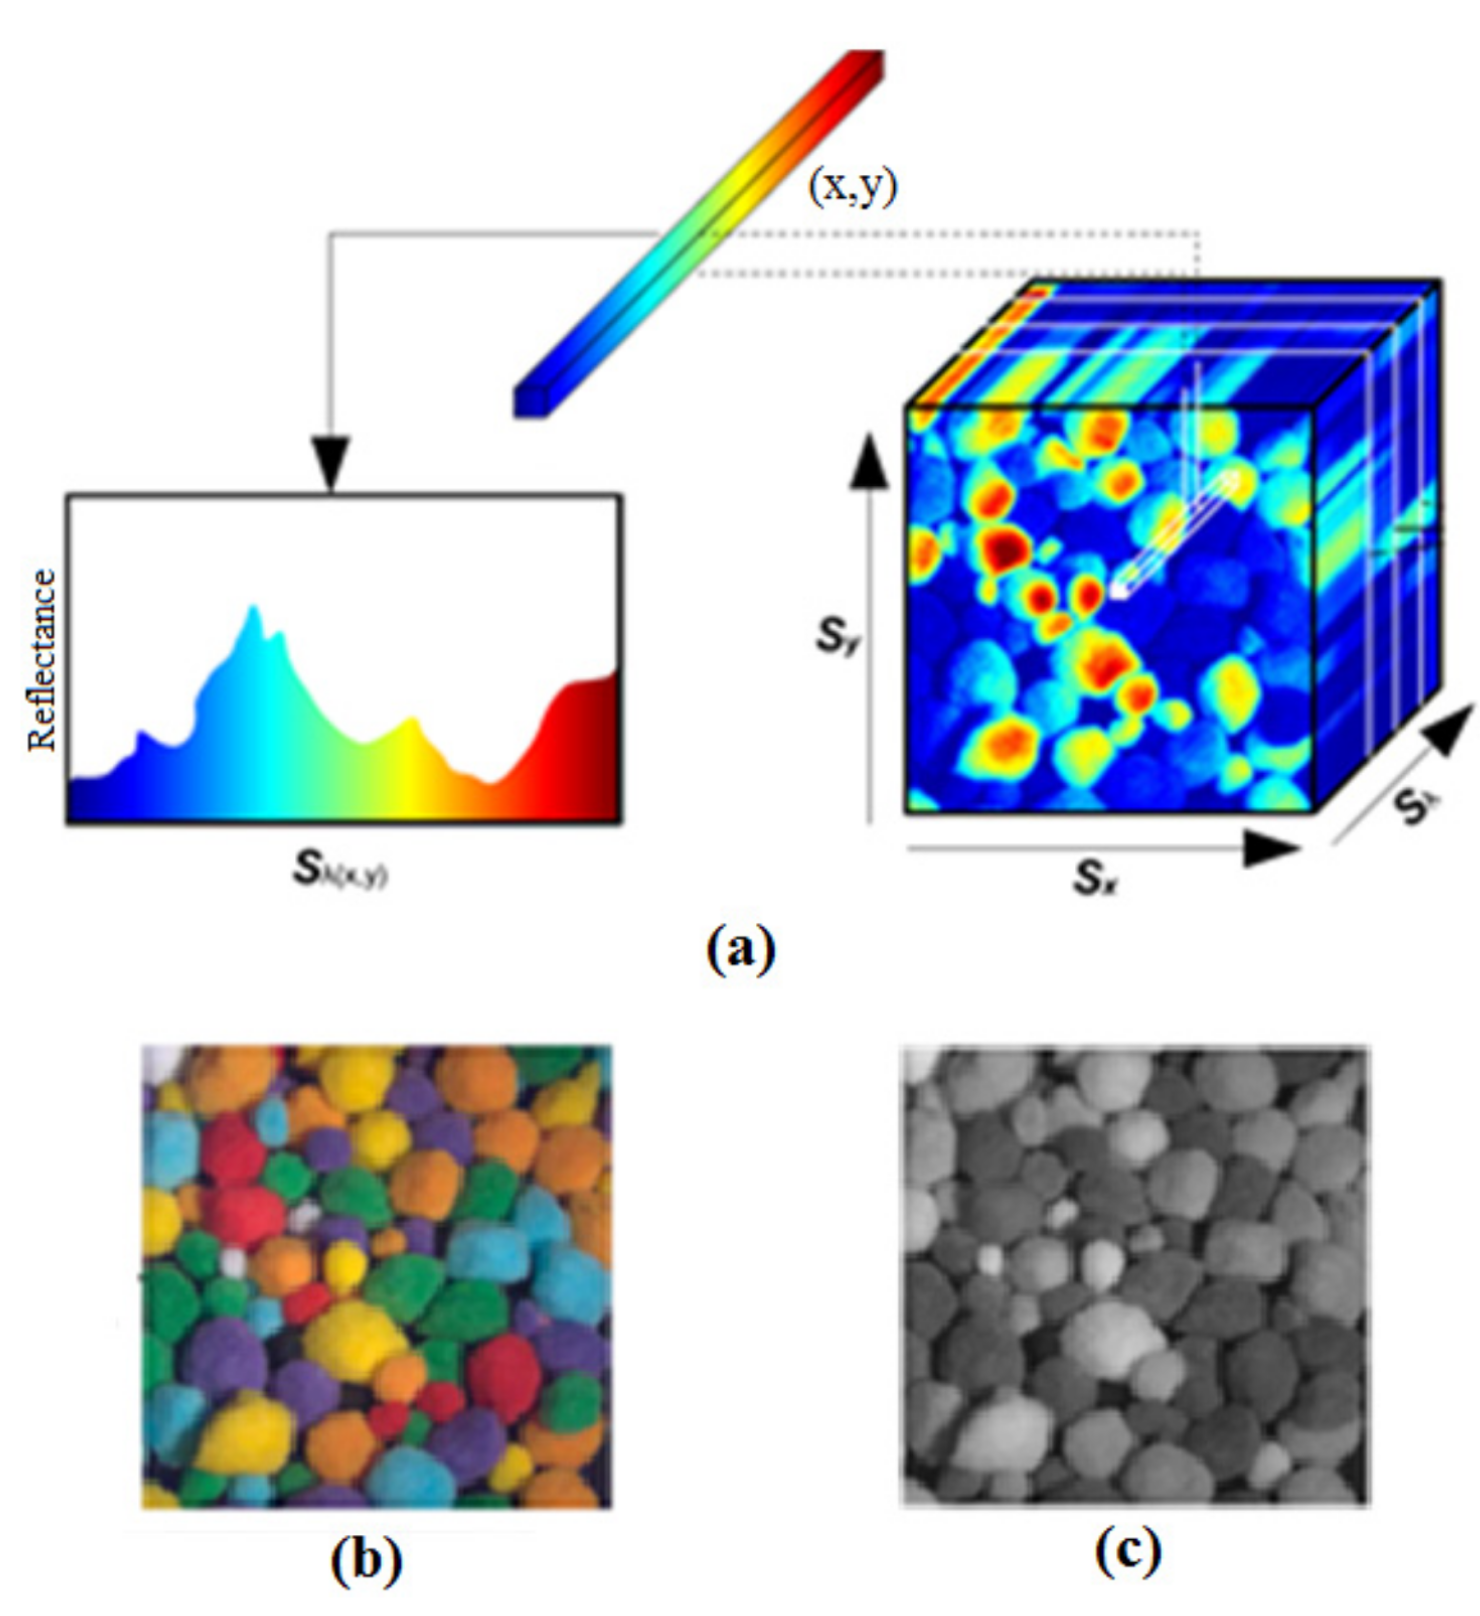
\includegraphics[width=1\linewidth]{figures/HSI_example.png}
            \captionsetup{labelformat=simple, labelsep=colon, font=scriptsize, labelfont={color=gray,bf}}
            \caption{(a) HSI Cube; (b) RGB Image; (c) Grayscale Image. \cite{khanModernTrendsHyperspectral2018}}
            \label{fig:khan-modern}
            \end{figure}
        \end{column}

        % Right column
        \begin{column}{0.62\textwidth}
            \begin{itemize}
                \item \textbf{Hyperspectral Images (HSIs)}: 
                \begin{itemize}
                    \item Capture spatial \& spectral properties.
                \end{itemize}
                \vspace{0.2cm}
                \item \textbf{Why Unsupervised Clustering?} 
                \begin{itemize}
                    \item Reveal hidden patterns
                    \item No need for labeled data
                \end{itemize}
                \vspace{0.2cm}
                \item \textbf{Challenges in HSIs:}
                \begin{itemize}
                    \item High dimensionality
                    \item Spectral/spatial variability
                    \item Noise \& distortions
                \end{itemize}
            \end{itemize}
        \end{column}
    \end{columns}
\end{frame}

%%% Local Variables:
%%% mode: latex
%%% TeX-master: "../topic-slide-main"
%%% End:
% \input{sections/state-of-the-art}

%% ----------- Method

% \input{sections/bluered-dcp-v2}
% \input{sections/bluered-har-v2}
% \input{sections/bluered-phase}

%% ----------- Algorithm 

%%
%% bluered-alg-formal.tex
%%


\begin{frame}{BlueRed: algorithm DT(I)}

\begin{columns}
%% double-column layout 
\begin{column}{0.45\textwidth}                 %% Left Column 

{\small \bf Descending Triangulation (I)}
% 
\begin{overprint}
\onslide<1>\scalebox{0.7}{
\begin{minipage}{1.5\textwidth}
    % !TEX root = ../digraph-main.tex

\renewcommand{\thealgocf}{}
\begin{algorithm}[H]
  \small
\SetKwInOut{Input}{Input}
\SetKwInOut{Output}{Output}
\SetKwRepeat{Do}{do}{while}
\SetKwFunction{filter}{filter}
{\bf Input:} $h$\,
// standardized clustering function with d.m. property
\\
\phantom{{\bf Input:}} $G$
//  weakly connected digraph
\\
{\bf Output:}  ${\cal B}_{\min} = ({\cal B}_{\Omega}, {\cal B}_{\theta})$  
// a pair of ordered lists
\\
{\bf Initialization:}
${\cal B}_{\Omega} \gets \{\Omega_V, \Omega_v\}, \, 
{\cal B}_{\theta} \gets \{0, \pi/4, \pi/2\}$
\\[0.1em]
\phantom{{\bf Initialization:}}
$\mbox{\rm T}  \gets \{\,\overline{\Omega_V \Omega_v}\, \}$
// candidate line-segment set

\While{\rm T $\neq \emptyset$ } {
  $ \ell = \overline{ \Omega_{a}\Omega_{b} }   \gets
  {\tt getSegment}(\, \mbox{\rm T} \,) $
  \\ 
  $\mbox{\rm T} \gets \mbox{\rm T} - \ell; \,\quad
  \gamma_{\ell} \gets -1/{\tt slope}(\,\ell\,); \,\quad
  \theta_{\ell} \gets {\rm atan}(\gamma_{\ell})$
  \\
  $ \Omega_{\ell} \gets
  \argmin\{ h(\Omega,\gamma_{\ell}) \mid \Omega \in \mathcal{L}(G) \} $ 
  \\
  \If{ $ {\tt offSegment}(\ell, \Omega_\ell) $ }
  {
    $\mbox{\rm T}_{\phantom{\theta}}\, \gets
    \mbox{\rm T} \cup
    \{ \overline{\Omega_{a}\Omega_{\ell}},  \overline{\Omega_{\ell}\Omega_{b}} \}$
    \\
    $\theta_{\rm a{\ell}} \gets 
      {\rm atan}
      \left( 
        -1 / {\tt slope}( \overline{\Omega_a \Omega_{\ell}} ) 
      \right)$ 
    \\
    $\theta_{\rm {\ell}b} \gets 
      {\rm atan}
      \left( 
        -1 / {\tt slope}( \overline{\Omega_{\ell} \Omega_b} )
      \right)$
    \\
    $ {\cal B}_{\theta}\, \gets {\tt insert}(
      {\cal B}_{\theta},
      \{ \theta_{\rm a{\ell}}, \theta_{\rm {\ell}b} \}
     ); \,\,\,
     {\cal B}_{\theta} \gets {\cal B}_{\theta}- \{\theta_{\rm \ell}\}$
    \\
    ${\cal B}_{\Omega} \gets {\tt insert}( {\cal B}_{\Omega}, \Omega_{\ell} )$
  } % End of IF 
} % End of WHILE
%
%\textcolor{red}{\em problem with updating} $\Theta$ in ${\cal B}_\min$ 
\end{algorithm}

\end{minipage}
}
\end{overprint}

\vspace*{0.5em}

{\small \bf DT(I) properties:}
  \begin{list}{$\ast$}{\itemsep = -1pt \leftmargin = 10pt}
    \footnotesize 
	\item fully autonomous, in $p$ steps
	\item theoretically guaranteed to reach ${\cal B}_{\min}$
	\item low complexity: $p\!$ $\times\!$ cost ($\gamma$-specific search)
	\item simple, efficient: successive triangulation steps
\end{list}
% 
\end{column}

\hspace*{4em}                                                          %%  make space between columns 

\begin{column}{0.42\textwidth}                                %% Right Column 
  %
  Five points: 
  \begin{enumerate}
  \item problem description, including preliminary when necessary 
  \item state of the art, citing notable  related work,
     knowledge or technology gaps 
  \item method description 
  \item analytical, experimental evidence, claims 
  \item discussion: advance made, potential promised, remaining limitation, lessons learned 
  \end{enumerate}
 %  
\end{column}
%
\end{columns}   %% End of multiple columns 
% 
\end{frame}

%%
%%
%% 

% \input{sections/bluered-alg-informal}

%% ----------- Experiments

% \input{sections/exp-polblogs}
% \input{sections/exp-mnist}
% \input{sections/exp-citation}

%% ----------- Discussion

% \input{sections/discussion}


%% -----------  Acknowledgement

% !TEX root = ../digraph-main.tex

\begin{frame}{Acknowledgements}

  \begin{columns}
    \begin{column}{0.35\textwidth}
      We thank xxx for xxx 
    \end{column}
    \hspace*{2em}
    \begin{column}{0.45\textwidth}
      This work is supported in part by
      \begin{list}{$\diamond$}{\itemsep = 3pt \leftmargin=10pt}
        \item research grant xxxx
        \item research grant xxxx 
      \end{list}
    \end{column}
  \end{columns}

\end{frame}



%% ============ BIBLIOGRAPHY
\appendix

\begin{frame}[noframenumbering,plain,allowframebreaks]{Bibliography}
    \printbibliography[heading=none]
\end{frame}


\end{document}


%%%%

%%%%  provided by Xiaobai Sun 
%%%%
